\documentclass{article}
\usepackage[utf8]{inputenc}
\usepackage[brazil]{babel}
\usepackage[a4paper, top=2.5cm, bottom=2.5cm, left=2cm, right=2.5cm]{geometry}
\usepackage{makecell}

\usepackage{pgf}
\usepackage{tikz}
\usetikzlibrary{arrows,automata}

\usepackage{graphicx}
\graphicspath{{figures/}}

\usepackage{amsmath,amssymb}
\DeclareMathOperator*{\argmax}{argmax}

\linespread{1.3}
\setlength{\parindent}{4em}
\setlength{\parskip}{0.75em}

% PB: redefinir maketitle
\makeatletter
\def\@maketitle
{
    \begin{flushleft}
        \let \footnote \thanks
        {\Large \textbf{\@title} \par}
        %\vskip 0.5em
        {\large \textbf{\@author} \par}
        %\vskip 0.5em
        {\large \textit{\@date}}
    \end{flushleft}
    \par
    \vskip 1.5em
}
\makeatother

\tikzset{
    state-node/.style={
        fill=none, shape=circle, draw=black, thick, text=black, minimum size=0.6cm},
    action-node/.style={
        fill=black, draw=none, text=white, shape=circle, inner sep=0.05cm, minimum size=0.2cm},
    reward-node/.style={
        fill=none, draw=black, text=black},
    hidden-node/.style={
        fill=none, draw=none, text=white, shape=circle, inner sep=0,outer sep=0, minimum size=0.0cm},
    action-label/.style={
        shape=circle, text=white, draw=none, fill=black, inner sep=0.05cm, minimum size=0.2cm, align=center, yshift=0.0cm, anchor=center},
    reward-label/.style={
        shape=rectangle, text=black, draw=black, fill=white, minimum size=0.5cm, align=center, yshift=0.0cm, anchor=center},
    hidden-edge/.style={
        text=white, draw=none, fill=none, inner sep=0,outer sep=0, minimum size=0.0cm},
}

\newcommand{\todo}[1]{ --\textcolor{red}{\textbf{#1}}--}
%\newcommand{\todo}[1]{}

\newcommand{\simplebandit}{
    \begin{tikzpicture}[->,>=stealth', auto, node distance=1.5cm]
        \node[state-node]  (SimpleBanditS1) {$s$};
        \node[reward-node] (SimpleBanditR1) [below of=SimpleBanditS1, xshift=-1.0cm] {$r$};
        \node[reward-node] (SimpleBanditR2) [below of=SimpleBanditS1, xshift=0.0cm]  {$r$};
        \node[reward-node] (SimpleBanditR3) [below of=SimpleBanditS1, xshift=1.0cm]  {$r$};
        
        \draw[bend right] (SimpleBanditS1) to node[action-label] {$a$} (SimpleBanditR1);
        \draw             (SimpleBanditS1) to node[action-label] {$a$} (SimpleBanditR2);
        \draw[bend left]  (SimpleBanditS1) to node[action-label] {$a$} (SimpleBanditR3);
    \end{tikzpicture}
}
    
\title{Aprendizado por Reforço}
\author{Aula 02 - Exemplo com um único estado}
\date{Paulo Bruno de Sousa Serafim - Outubro 2019}

\begin{document}

\maketitle

\section{\textit{Multi-armed bandit}}

    Vamos imaginar o caso mais simples, em que só temos um único estado. Assim a dinâmica de interação é bem simples, escolhemos uma ação e recebemos uma recompensa por ela. Nesse caso, só temos que nos preocupar com qual ação tomar imediatamente e com a sua recompensa. Se existirem k ações possíveis, podemos executar qualquer uma delas e receberemos uma recompensa. O diagrama a seguir representa essa dinâmica:

    \todo{diagrama com um único estado}

    \textit{O caso em que temos somente um estado é um problema bem conhecido e chamado de "Multi-Armed Bandit" (adicionar nota: a tradução para ``one-armed bandit'' é máquina caça-níquel, então ``multi-armed bandit'' seria uma máquina caça-níquel com múltiplas alavancas).}
    
    Esse é um problema bem conhecido e muito estudado na literatura: k-armed bandit [nota tradução máquina caça-níquel]. Imagine que você vá jogar em máquinas caça-níquel. Cada máquina dará resultados diferentes com probabilidades diferentes, mas você tem um documento contendo os valores ganhos possíveis e suas probabilidades para cada máquina. Você só pode jogar uma única vez. Qual máquina você escolheria?

    \begin{center}
    \begin{tikzpicture}[-, >=stealth', auto, node distance=1.5cm]
        \node[state-node] (S1) {$s$};
        \node[action-node] (A1) [below of=S1, xshift=-2.0cm] {$a_1$};
        \node[action-node] (A2) [below of=S1, xshift=2.0cm]  {$a_2$};
        \node[reward-node] (R1) [below of=A1, xshift=-1.0cm] {$r_1$};
        \node[reward-node] (R2) [below of=A1, xshift=0.0cm]  {$r_2$};
        \node[reward-node] (R3) [below of=A1, xshift=1.0cm]  {$r_3$};
        \node[reward-node] (R4) [below of=A2, xshift=0.0cm]  {$r_4$};
        
        \draw[bend right=40] (S1) to node[left]  {} (A1);
        \draw[bend left=40]  (S1) to node[right] {} (A2);
        \draw[bend right]    (A1) to node[left]  {$p_{11}$} (R1);
        \draw                (A1) to node[left]  {$p_{12}$} (R2);
        \draw[bend left]     (A1) to node[right] {$p_{13}$} (R3);
        \draw                (A2) to node[right] {$p_{21}$} (R4);
    \end{tikzpicture}
    \end{center}

    A escolha ótima, i.e., a escolha racional que potencialmente dará o maior valor é aquela cujo retorno esperado é o maior. Em outras palavras, você deve escolher a máquina cujo valor esperado seja o maior. Lembrando que estamos considerando que uma máquina é uma ação, podemos representar essa escolha da seguinte forma:
    
    Valor de uma máquina \textit{a} = Valor esperado do retorno ao jogar a máquina \textit{a}
    
    De outra forma:
    
    \begin{equation}
        q_*(a) \ \dot{=} \ \mathbb{E}[R_t \mid A_t = a]
    \end{equation}

    \subsection{Descrição informal}
    
    \subsection{Formalização}

\section{Dilema \textit{``Exploration vs. Exploitation''}}

    Pegando emprestado um exemplo \todo{procurar onde vi esse exemplo, provavelmente sutton}, imagine que você goste bastante de uma lanchonete que tem um ótimo hambúrguer. Você pode continuar sempre indo na mesma lanchonete. Você sempre vai comer um ótimo hambúrguer, mas pode ser que exista outra lanchonete que tenha um hambúrguer ainda melhor, e você não vai saber. Você poderia decidir, por exemplo, nunca repetir uma lanchonete, assim você conheceria ótimas lanchonetes com ótimos hambúrguers, mas algumas vezes iria comer sanduíches ruins.
    
    Esse exemplo ilustra o dilema entre sempre escolher uma boa opção (a mesma lanchonete), ou seja, \textbf{explorar} aquilo que já é conhecido, e prospectar (mudar de lanchonete), ou seja, testar outras opções ainda não verificadas. 

    \subsection{Definições}
    
        \subsection{\textit{``Exploration''} = Prospecção}
        
        \subsection{\textit{``Exploitation''} = Exploração}
    
    \subsection{Estratégias}
    
        As estratégias para lidar com o dilema anterior se baseiam em executar ações de maneira gulosa na maior parte do tempo, mas ainda executar ações não-gulosas algumas vezes.
    
        \subsubsection{Estratégias $\epsilon$}
        
            \begin{itemize}
                \item \textbf{$\epsilon$-greedy}: executa a ação gulosa em uma porcentagem $(1-\epsilon)$ e executa uma ação aleatória $\epsilon$.
                \item \textbf{$\epsilon$-first}: para um conjunto N de ações, executa $(1 - \epsilon N)$ ações gulosas e executa $(\epsilon N)$ ações não-gulosas.
                \item \textbf{$\epsilon$-decay}: No início do aprendizado não há ainda uma boa distribuição das recompensas, de modo que os valores tendem a ser menos confiáveis, assim faz sentido prospectar ações. Após algumas iterações a recompensa já terá sido mais distribuída, de modo que faz sentido termos uma fase de exploração maior. Após várias iterações a distribuição de recompensa será bem mais confiável, logo a fase de exploração deverá ser máxima. Essa estratégia é representada usando um $\epsilon_{I}$ alto nas primeiras $I$ iterações (possivelmente $1$), um $\epsilon_{F}$ bem baixo a partir da iteração $F$ e um $\epsilon$ que diminui (decai) de $\epsilon_{I}$ a $\epsilon_{F}$ entre $I$ e $F$. O tipo de decaimento mais comum é o linear, representado na Figura \ref{fig:epsilon-decay}, com $\epsilon_{I} = 1.0$, $\epsilon_{F} = 0.1$, $I = 6$ e $F = 31$.
                
                \begin{figure}[ht]
                    \centering
                    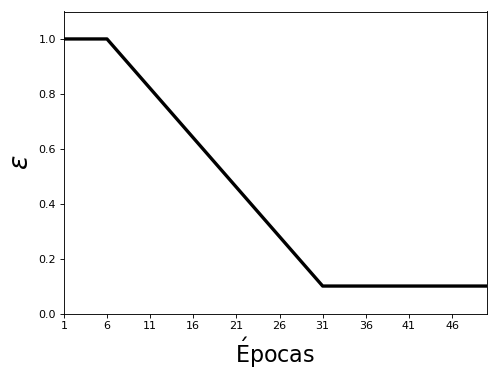
\includegraphics[width=200pt]{epsilon-decay.png}
                    \caption{\todo{fazer o grafico usando tikz} Fonte:}
                    \label{fig:epsilon-decay}
                \end{figure}
            \end{itemize}
        
\section{Função valor-ação}

    Função valor-ação ótima:

    \begin{equation}
        q_*(a) \ \dot{=} \ \mathbb{E}[R_t \mid A_t = a]
    \end{equation}

    Escolha gulosa:

    \begin{equation}
        A_t \ \dot{=} \ \argmax_a Q_t(a)
    \end{equation}
    
    \begin{center}
    \begin{tikzpicture}[->,>=stealth', auto, node distance=4.0cm, thick]
        \node[state-node]  (S1) {$s_1$};
        \node[state-node]  (S2) [below of=S1, xshift=-3.0cm] {$s_2$};
        \node[state-node]  (S3) [below of=S1, xshift= 3.0cm] {$s_3$};
        \node[hidden-node] (A1) [above of=S2, yshift=-1.5cm] {};
        \node[hidden-node] (A2) [below of=S1, yshift=2.5cm]  {};
        
        \draw[bend right=20,-] (S1) to node[action-label]           {$a_1$} (A1);
        \draw[-]               (S1) to node[action-label, pos=0.4]  {$a_2$} (A2);
        \draw[bend left=40]    (S1) to node[action-label, pos=0.25] {$a_3$} (S3);
        
        \draw[bend right=30]   (A1) to node[left, pos=0.2]  {$p_1$} (S2);
        \draw[bend left=30]    (A1) to node[right, pos=0.2] {$p_2$} (S2);
        \draw[bend left=40]    (A2) to node[left, pos=0.3]  {$p_3$} (S2);
        \draw[bend right=40]   (A2) to node[right, pos=0.3] {$p_4$} (S3);
        
        \draw[hidden-edge, bend right=30] (A1) to node[reward-label]           {$r_1$} (S2);
        \draw[hidden-edge, bend left=30]  (A1) to node[reward-label]           {$r_2$} (S2);
        \draw[hidden-edge, bend left=40]  (A2) to node[reward-label]           {$r_3$} (S2);
        \draw[hidden-edge, bend right=40] (A2) to node[reward-label]           {$r_4$} (S3);
        \draw[hidden-edge, bend left=40]  (S1) to node[reward-label, pos=0.65] {$r_5$} (S3);
    \end{tikzpicture}
    \end{center}
    
    Para simplificar o grafo, na maioria das vezes os nós das ações serão omitidos e as ações serão indicadas nos rótulos das arestas. Além disso, se a probabilidade for 1, ela é omitida.
    
    \subsection{Definição}
    
    \subsection{Versão incremental}
        
        \begin{equation}
            Q_n \ \dot{=} \ \frac{R_1 + R_2 + \cdots + R_{n-1}}{n - 1}
        \end{equation}
        
        \begin{equation}
        \begin{split}
            Q_{n+1} & \ \dot{=} \ \frac{1}{n} \sum_{i=1}^{n} R_i \\
            & = \ Q_n + \frac{1}{n} \Big[ R_n - Q_n \Big]
        \end{split}
        \end{equation}
        
        Ver no livro a derivação dessa equação (eq. 2.3).
        
        \begin{equation}
            NovaEstimativa \leftarrow AntigaEstimativa + TamanhoPasso \Big[ Objetivo - AntigaEstimativa \Big]
        \end{equation}
        
        \begin{equation}
        \begin{split}
            Q_{n+1} & \ \dot{=} \ Q_n + \alpha \Big[ R_n - Q_n \Big] \\
            & = \ (1 - \alpha)^n Q_1 + \sum_{i=1}^{n} \alpha (1 - \alpha)^{n - i} R_i
        \end{split}
        \end{equation}
        
    \subsection{Escolha dos valores iniciais}
        
        Obs.: citar a diferença entre problemas estacionários e não-estacionários
        
        \subsubsection{Valores otimistas}
        
        \subsubsection{Limite Superior de Confiança (UCB)}
        
\section{Nonassociative, Associative, Full RL Problem}

    \subsection{Nonassociative}
    
        \begin{center}
            \simplebandit
        \end{center}

    \subsection{Associative}

        \begin{center}
        \begin{tikzpicture}[]
            \node[draw=black] (AB1) {
                \begin{tikzpicture}[]
                    \node[] (B1) {
                        \simplebandit
                    };
                    \node[right of=B1, xshift=2.0cm] (B2) {
                        \simplebandit
                    };
                    \node[right of=B2, xshift=2.0cm] (B3) {
                        \simplebandit
                    };
                    \node[right of=B3, xshift=1.0cm] (B4) {
                        $\boldsymbol{\cdots}$
                    };
                    \node[right of=B4, xshift=1.0cm] (B5) {
                        \simplebandit
                    };
                \end{tikzpicture}
            };
            
            \node[draw=red, below of=AB1, yshift=-2.0cm] (AB2) {
                \begin{tikzpicture}[]
                    \node[] (B1) {
                        \simplebandit
                    };
                    \node[right of=B1, xshift=2.0cm] (B2) {
                        \simplebandit
                    };
                    \node[right of=B2, xshift=2.0cm] (B3) {
                        \simplebandit
                    };
                    \node[right of=B3, xshift=1.0cm] (B4) {
                        $\boldsymbol{\cdots}$
                    };
                    \node[right of=B4, xshift=1.0cm] (B5) {
                        \simplebandit
                    };
                \end{tikzpicture}
            };
            
            \node[draw=blue, below of=AB2, yshift=-1.0cm] (AB3) {
                $\Huge\vdots$
            };
        
            \node[draw=green, below of=AB3, yshift=-1.0cm] (AB4) {
                \begin{tikzpicture}[]
                    \node[] (B1) {
                        \simplebandit
                    };
                    \node[right of=B1, xshift=2.0cm] (B2) {
                        \simplebandit
                    };
                    \node[right of=B2, xshift=2.0cm] (B3) {
                        \simplebandit
                    };
                    \node[right of=B3, xshift=1.0cm] (B4) {
                        $\boldsymbol{\cdots}$
                    };
                    \node[right of=B4, xshift=1.0cm] (B5) {
                        \simplebandit
                    };
                \end{tikzpicture}
            };
            
            \draw[->, thick] (AB1) to node {} (AB2);
            \draw[->, thick] (AB2) to node {} (AB3);
            \draw[->, thick] (AB3) to node {} (AB4);
        \end{tikzpicture}
        \end{center}
        
        
    \subsection{Full RL Problem}
    
        \begin{center}
        \begin{tikzpicture}[]
            \node[draw=black] (RL1) {
                \begin{tikzpicture}[]
                    \node[] (SB1) {
                        \begin{tikzpicture}[-,>=stealth', auto, node distance=1.5cm]
                            \node[state-node]  (SB1S1) {$s$};
                            \node[reward-node] (SB1R1) [below of=SB1S1, xshift=-1.0cm] {$r$};
                            \node[reward-node] (SB1R2) [below of=SB1S1, xshift=0.0cm]  {$r$};
                            \node[reward-node] (SB1R3) [below of=SB1S1, xshift=1.0cm]  {$r$};
                            
                            \draw[bend right] (SB1S1) to node[action-label] {$a$} (SB1R1);
                            \draw             (SB1S1) to node[action-label] {$a$} (SB1R2);
                            \draw[bend left]  (SB1S1) to node[action-label] {$a$} (SB1R3);
                        \end{tikzpicture}
                    };
                    
                    \node[right of=SB1, xshift=2.0cm] (SB2) {
                        \begin{tikzpicture}[-,>=stealth', auto, node distance=1.5cm]
                            \node[state-node]  (SB2S1) {$s$};
                            \node[reward-node] (SB2R1) [below of=SB2S1, xshift=-1.0cm] {$r$};
                            \node[reward-node] (SB2R2) [below of=SB2S1, xshift=0.0cm]  {$r$};
                            \node[reward-node] (SB2R3) [below of=SB2S1, xshift=1.0cm]  {$r$};
                            
                            \draw[bend right] (SB2S1) to node[action-label] {$a$} (SB2R1);
                            \draw             (SB2S1) to node[action-label] {$a$} (SB2R2);
                            \draw[bend left]  (SB2S1) to node[action-label] {$a$} (SB2R3);
                        \end{tikzpicture}
                    };
                    
                    \node[right of=SB2, xshift=1.0cm] (DOTS1) {
                        $\boldsymbol{\cdots}$
                    };
                    
                    \node[right of=DOTS1, xshift=1.0cm] (SB3) {
                        \begin{tikzpicture}[-,>=stealth', auto, node distance=1.5cm]
                            \node[state-node]  (SB3S1) {$s$};
                            \node[reward-node] (SB3R1) [below of=SB3S1, xshift=-1.0cm] {$r$};
                            \node[reward-node] (SB3R2) [below of=SB3S1, xshift=0.0cm]  {$r$};
                            \node[reward-node] (SB3R3) [below of=SB3S1, xshift=1.0cm]  {$r$};
                            
                            \draw[bend right] (SB3S1) to node[action-label] {$a$} (SB3R1);
                            \draw             (SB3S1) to node[action-label] {$a$} (SB3R2);
                            \draw[bend left]  (SB3S1) to node[action-label] {$a$} (SB3R3);
                        \end{tikzpicture}
                    };
                \end{tikzpicture}
            };
            
            \node[draw=red, below of=RL1, yshift=-2.0cm] (RL2) {
                \begin{tikzpicture}[remember picture]
                    \node[] (SB4) {
                        \begin{tikzpicture}[-,>=stealth', auto, node distance=1.5cm]
                            \node[state-node]  (SB4S1) {$s$};
                            \node[reward-node] (SB4R1) [below of=SB4S1, xshift=-1.0cm] {$r$};
                            \node[reward-node] (SB4R2) [below of=SB4S1, xshift=0.0cm]  {$r$};
                            \node[reward-node] (SB4R3) [below of=SB4S1, xshift=1.0cm]  {$r$};
                            
                            \draw[bend right] (SB4S1) to node[action-label] {$a$} (SB4R1);
                            \draw             (SB4S1) to node[action-label] {$a$} (SB4R2);
                            \draw[bend left]  (SB4S1) to node[action-label] {$a$} (SB4R3);
                        \end{tikzpicture}
                    };
                    
                    \node[right of=SB4, xshift=2.0cm] (SB5) {
                        \begin{tikzpicture}[-,>=stealth', auto, node distance=1.5cm]
                            \node[state-node]  (SB5S1) {$s$};
                            \node[reward-node] (SB5R1) [below of=SB5S1, xshift=-1.0cm] {$r$};
                            \node[reward-node] (SB5R2) [below of=SB5S1, xshift=0.0cm]  {$r$};
                            \node[reward-node] (SB5R3) [below of=SB5S1, xshift=1.0cm]  {$r$};
                            
                            \draw[bend right] (SB5S1) to node[action-label] {$a$} (SB5R1);
                            \draw             (SB5S1) to node[action-label] {$a$} (SB5R2);
                            \draw[bend left]  (SB5S1) to node[action-label] {$a$} (SB5R3);
                        \end{tikzpicture}
                    };
                    
                    \node[right of=SB5, xshift=1.0cm] (DOTS2) {
                        $\boldsymbol{\cdots}$
                    };
                    
                    \node[right of=DOTS2, xshift=1.0cm] (SB6) {
                        \begin{tikzpicture}[-,>=stealth', auto, node distance=1.5cm]
                            \node[state-node]  (SB6S1) {$s$};
                            \node[reward-node] (SB6R1) [below of=SB6S1, xshift=-1.0cm] {$r$};
                            \node[reward-node] (SB6R2) [below of=SB6S1, xshift=0.0cm]  {$r$};
                            \node[reward-node] (SB6R3) [below of=SB6S1, xshift=1.0cm]  {$r$};
                            
                            \draw[bend right] (SB6S1) to node[action-label] {$a$} (SB6R1);
                            \draw             (SB6S1) to node[action-label] {$a$} (SB6R2);
                            \draw[bend left]  (SB6S1) to node[action-label] {$a$} (SB6R3);
                        \end{tikzpicture}
                    };
                \end{tikzpicture}
            };
        \end{tikzpicture}
        \end{center}
    
\end{document}
